% TikZ source fragment: activation_swiglu.tex
% Included by % TikZ source fragment: activation_swiglu.tex
% Included by % TikZ source fragment: activation_swiglu.tex
% Included by % TikZ source fragment: activation_swiglu.tex
% Included by \input{figures/activation_swiglu}.
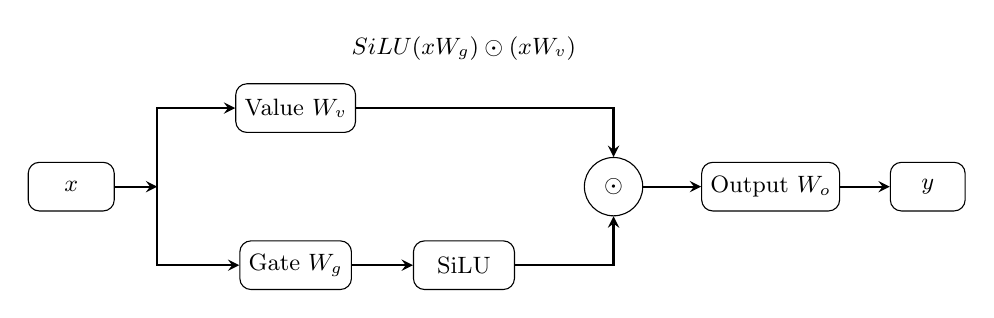
\begin{tikzpicture}[>=stealth, scale=0.95, transform shape, every node/.style={font=\small}]
    \node[draw, rounded corners, minimum width=1.15cm, minimum height=0.65cm]
        (x) at (0,0) {$x$};

    \coordinate (split) at (1.15,0);
    \draw[->, thick] (x) -- (split);

    \node[draw, rounded corners, minimum width=1.45cm, minimum height=0.65cm]
        (wv) at (3.0,1.05) {Value \(W_v\)};
    \node[draw, rounded corners, minimum width=1.45cm, minimum height=0.65cm]
        (wg) at (3.0,-1.05) {Gate \(W_g\)};

    \draw[->, thick] (split) |- (wv.west);
    \draw[->, thick] (split) |- (wg.west);

    \node[draw, rounded corners, minimum width=1.35cm, minimum height=0.65cm]
        (silu) at (5.25,-1.05) {SiLU};
    \draw[->, thick] (wg) -- (silu);

    \node[draw, circle, minimum size=0.78cm] (mul) at (7.25,0)
        {\(\odot\)};
    \draw[->, thick] (wv.east) -| (mul.north);
    \draw[->, thick] (silu.east) -| (mul.south);

    \node[draw, rounded corners, minimum width=1.55cm, minimum height=0.65cm]
        (wo) at (9.35,0) {Output \(W_o\)};
    \node[draw, rounded corners, minimum width=1.0cm, minimum height=0.65cm]
        (y) at (11.45,0) {$y$};
    \draw[->, thick] (mul) -- (wo);
    \draw[->, thick] (wo) -- (y);

    \node at (5.25,1.85)
        {\(\operatorname{SiLU}(xW_g)\odot(xW_v)\)};
\end{tikzpicture}
.
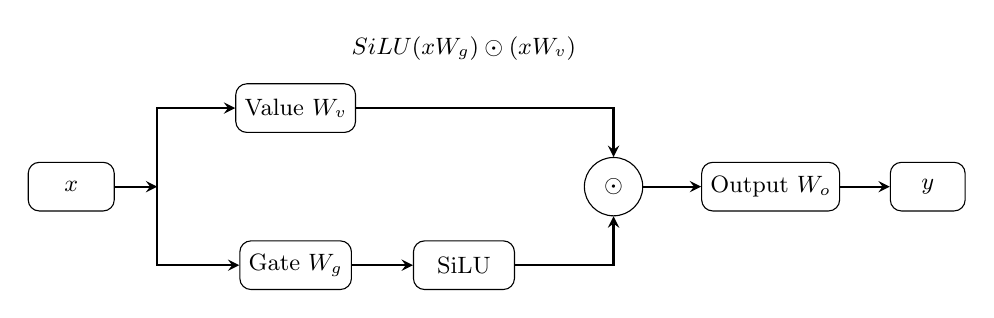
\begin{tikzpicture}[>=stealth, scale=0.95, transform shape, every node/.style={font=\small}]
    \node[draw, rounded corners, minimum width=1.15cm, minimum height=0.65cm]
        (x) at (0,0) {$x$};

    \coordinate (split) at (1.15,0);
    \draw[->, thick] (x) -- (split);

    \node[draw, rounded corners, minimum width=1.45cm, minimum height=0.65cm]
        (wv) at (3.0,1.05) {Value \(W_v\)};
    \node[draw, rounded corners, minimum width=1.45cm, minimum height=0.65cm]
        (wg) at (3.0,-1.05) {Gate \(W_g\)};

    \draw[->, thick] (split) |- (wv.west);
    \draw[->, thick] (split) |- (wg.west);

    \node[draw, rounded corners, minimum width=1.35cm, minimum height=0.65cm]
        (silu) at (5.25,-1.05) {SiLU};
    \draw[->, thick] (wg) -- (silu);

    \node[draw, circle, minimum size=0.78cm] (mul) at (7.25,0)
        {\(\odot\)};
    \draw[->, thick] (wv.east) -| (mul.north);
    \draw[->, thick] (silu.east) -| (mul.south);

    \node[draw, rounded corners, minimum width=1.55cm, minimum height=0.65cm]
        (wo) at (9.35,0) {Output \(W_o\)};
    \node[draw, rounded corners, minimum width=1.0cm, minimum height=0.65cm]
        (y) at (11.45,0) {$y$};
    \draw[->, thick] (mul) -- (wo);
    \draw[->, thick] (wo) -- (y);

    \node at (5.25,1.85)
        {\(\operatorname{SiLU}(xW_g)\odot(xW_v)\)};
\end{tikzpicture}
.
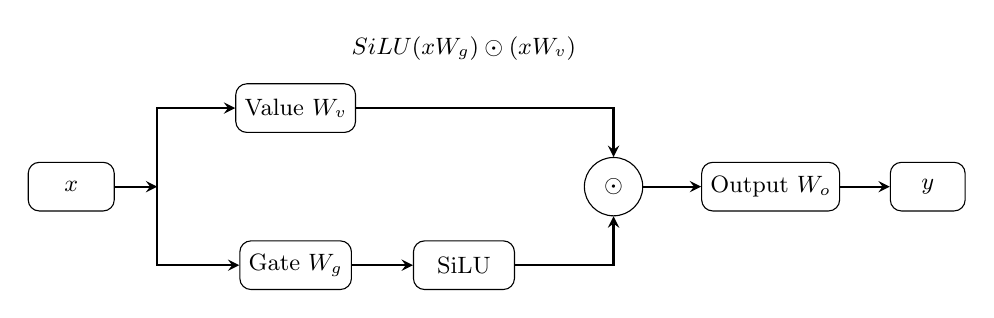
\begin{tikzpicture}[>=stealth, scale=0.95, transform shape, every node/.style={font=\small}]
    \node[draw, rounded corners, minimum width=1.15cm, minimum height=0.65cm]
        (x) at (0,0) {$x$};

    \coordinate (split) at (1.15,0);
    \draw[->, thick] (x) -- (split);

    \node[draw, rounded corners, minimum width=1.45cm, minimum height=0.65cm]
        (wv) at (3.0,1.05) {Value \(W_v\)};
    \node[draw, rounded corners, minimum width=1.45cm, minimum height=0.65cm]
        (wg) at (3.0,-1.05) {Gate \(W_g\)};

    \draw[->, thick] (split) |- (wv.west);
    \draw[->, thick] (split) |- (wg.west);

    \node[draw, rounded corners, minimum width=1.35cm, minimum height=0.65cm]
        (silu) at (5.25,-1.05) {SiLU};
    \draw[->, thick] (wg) -- (silu);

    \node[draw, circle, minimum size=0.78cm] (mul) at (7.25,0)
        {\(\odot\)};
    \draw[->, thick] (wv.east) -| (mul.north);
    \draw[->, thick] (silu.east) -| (mul.south);

    \node[draw, rounded corners, minimum width=1.55cm, minimum height=0.65cm]
        (wo) at (9.35,0) {Output \(W_o\)};
    \node[draw, rounded corners, minimum width=1.0cm, minimum height=0.65cm]
        (y) at (11.45,0) {$y$};
    \draw[->, thick] (mul) -- (wo);
    \draw[->, thick] (wo) -- (y);

    \node at (5.25,1.85)
        {\(\operatorname{SiLU}(xW_g)\odot(xW_v)\)};
\end{tikzpicture}
.
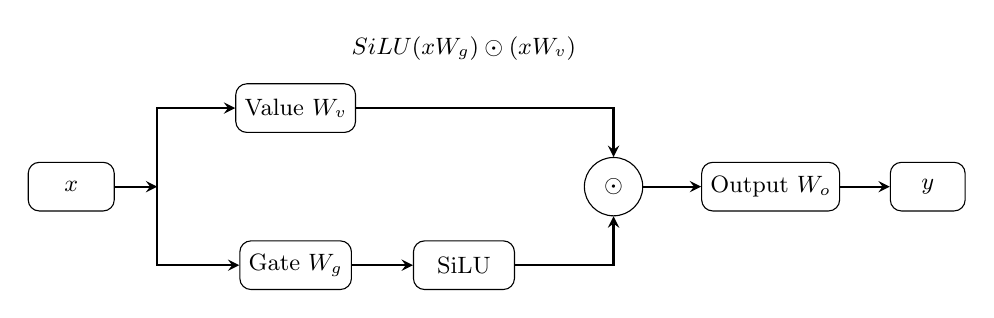
\begin{tikzpicture}[>=stealth, scale=0.95, transform shape, every node/.style={font=\small}]
    \node[draw, rounded corners, minimum width=1.15cm, minimum height=0.65cm]
        (x) at (0,0) {$x$};

    \coordinate (split) at (1.15,0);
    \draw[->, thick] (x) -- (split);

    \node[draw, rounded corners, minimum width=1.45cm, minimum height=0.65cm]
        (wv) at (3.0,1.05) {Value \(W_v\)};
    \node[draw, rounded corners, minimum width=1.45cm, minimum height=0.65cm]
        (wg) at (3.0,-1.05) {Gate \(W_g\)};

    \draw[->, thick] (split) |- (wv.west);
    \draw[->, thick] (split) |- (wg.west);

    \node[draw, rounded corners, minimum width=1.35cm, minimum height=0.65cm]
        (silu) at (5.25,-1.05) {SiLU};
    \draw[->, thick] (wg) -- (silu);

    \node[draw, circle, minimum size=0.78cm] (mul) at (7.25,0)
        {\(\odot\)};
    \draw[->, thick] (wv.east) -| (mul.north);
    \draw[->, thick] (silu.east) -| (mul.south);

    \node[draw, rounded corners, minimum width=1.55cm, minimum height=0.65cm]
        (wo) at (9.35,0) {Output \(W_o\)};
    \node[draw, rounded corners, minimum width=1.0cm, minimum height=0.65cm]
        (y) at (11.45,0) {$y$};
    \draw[->, thick] (mul) -- (wo);
    \draw[->, thick] (wo) -- (y);

    \node at (5.25,1.85)
        {\(\operatorname{SiLU}(xW_g)\odot(xW_v)\)};
\end{tikzpicture}
